\documentclass{article}
\usepackage{CJK}
\usepackage{ctex}
\usepackage{graphicx}
\usepackage{float}
\usepackage[colorlinks,linkcolor=black]{hyperref}
\graphicspath{{pic/}}
\renewcommand{\contentsname}{目录}
\title{动画导入与控制}
\author{杨铭 - 5130379022}
\begin{document}
\maketitle
\tableofcontents
\newpage
\section{概述}
本次作业主要使用\textbf{Unity}和\textbf{Blender}进行了简单的动画制作和导入控制。由于人物骨架动画的制作较为复杂,我使用了第三方的资源,而物体的动画为自己制作。
\section{资源说明}
\paragraph{}
本次主要使用了两个外部导入的模型、动作资源:
\begin{itemize}
  \item Unity-Chan
\end{itemize}
来自Unity社区Assets Store的3D模型+动画资源\href{https://www.assetstore.unity3d.com/cn/#!/content/18705}{Unity-Chan}是一个包含模型、动画、动画控制和三个预设场景的资源包。
我只使用了它的模型、动作和摄像机控制脚本。
\begin{figure}[H]
  \centering
  % Requires \usepackage{graphicx}
  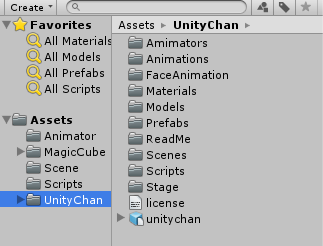
\includegraphics[width=10cm]{assets1.png}\\
  \caption{Unity-Chan}\label{1-1}
\end{figure}
\begin{itemize}
  \item MagicCube
\end{itemize}
这是一个我自己用Blender做的几个立方体运动的动画,通过位移,旋转设置关键帧,最后导出为.FBX文件
\begin{figure}[H]
  \centering
  % Requires \usepackage{graphicx}
  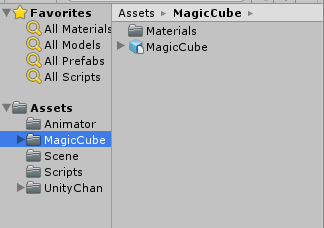
\includegraphics[width=10cm]{assets2.png}\\
  \caption{MagicCube1}\label{1-2}
  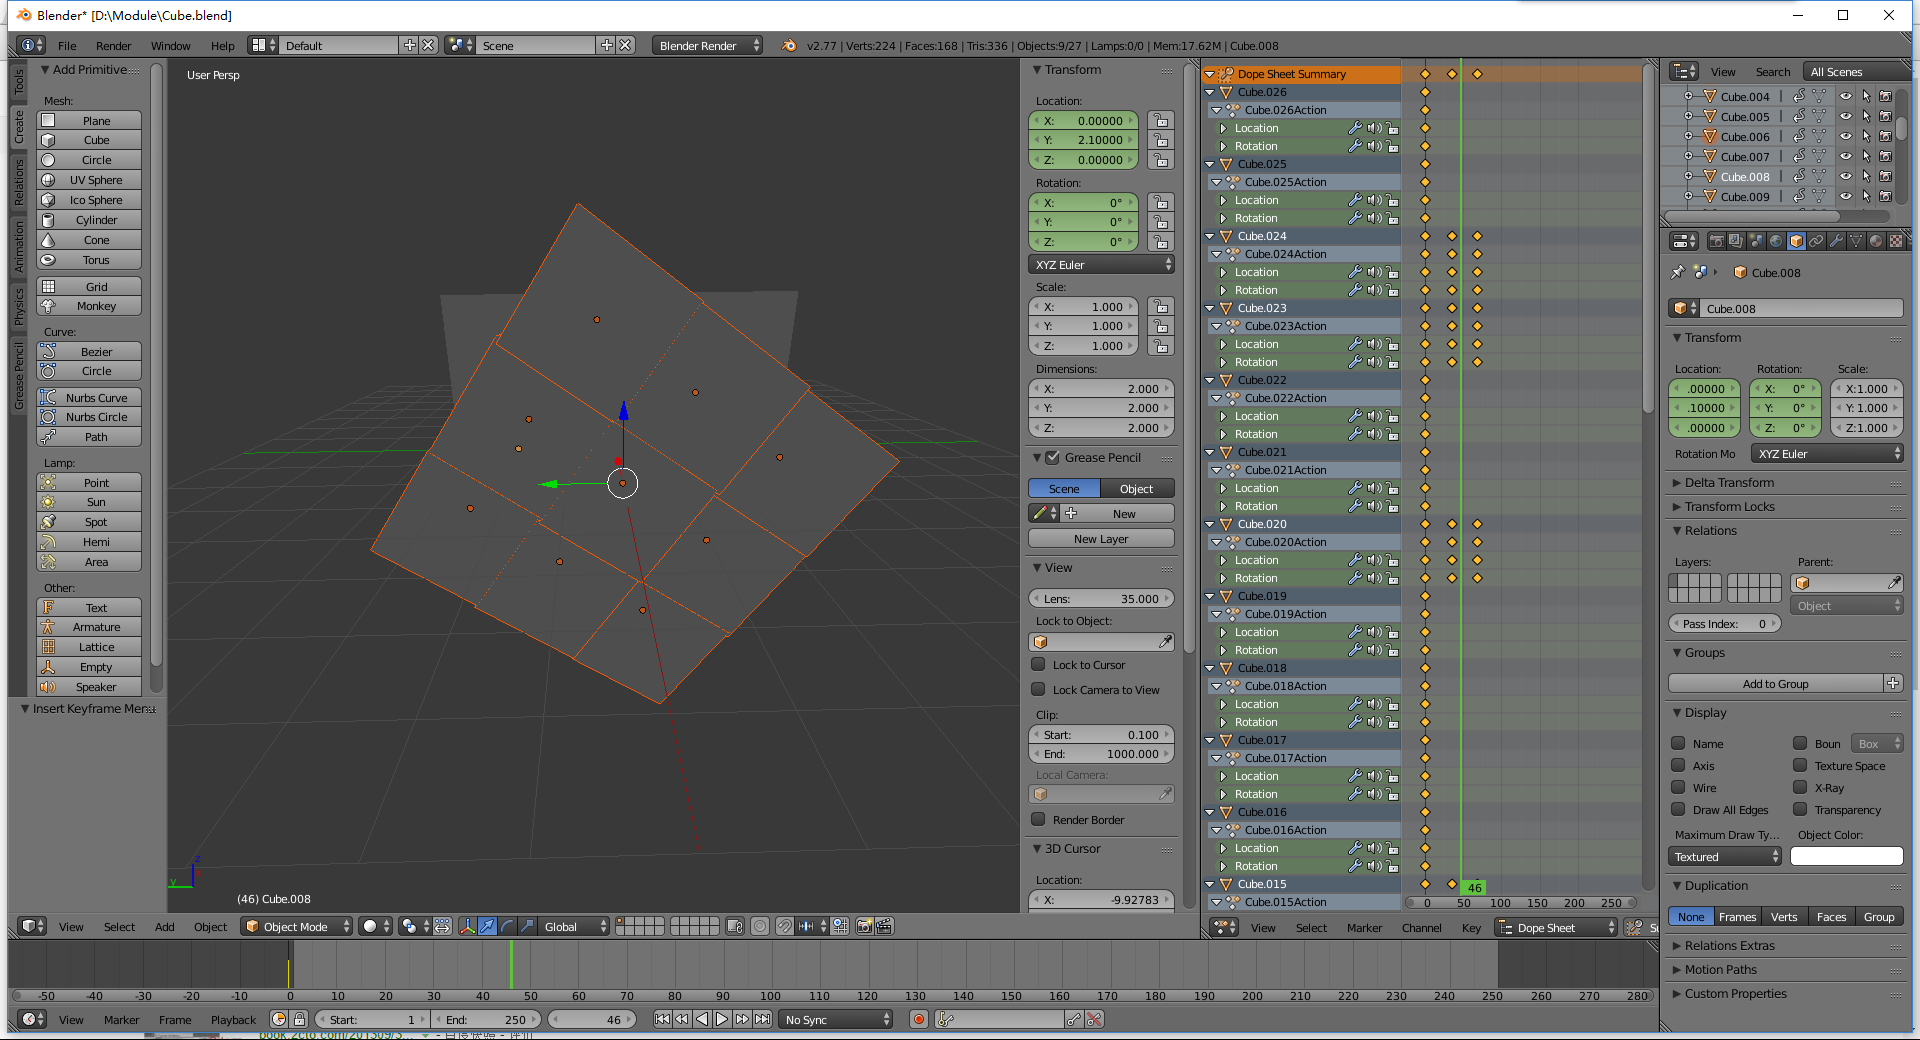
\includegraphics[width=36em]{blender1.png}\\
  \caption{MagicCube2}\label{1-3}
\end{figure}
\paragraph{}
在blender的导出时要注意将所有物体设置为某一个物体的子物体,并在导出设置的Animation里勾掉\textbf{all actions}选项,否则将会导出所有物体的所有动作,不方便在Unity里的设置。
\section{人物动画}
\subsection{简单动画导入}
\paragraph{}
首先将模型拖入场景,为它添加一个\textbf{Animator Controller},并将资源中自带的动画拖入Animator中
\begin{figure}[H]
  \centering
  % Requires \usepackage{graphicx}
  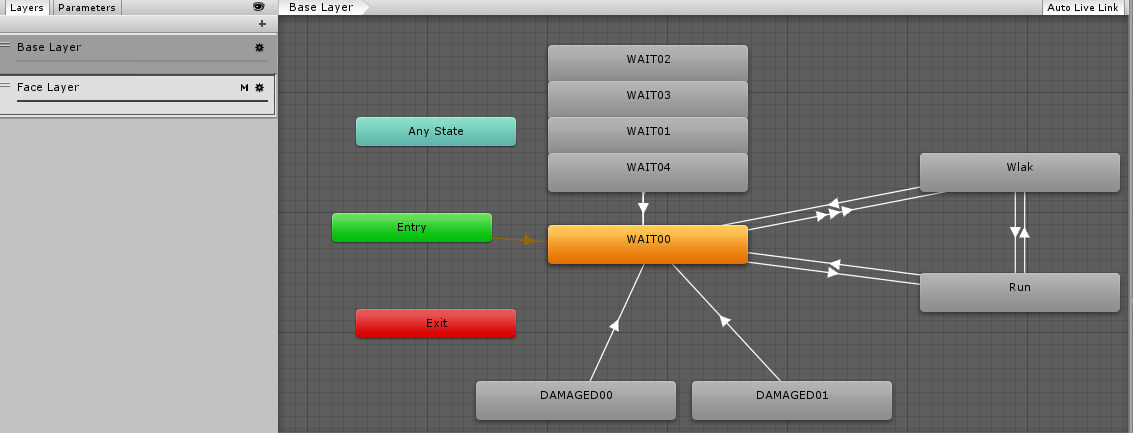
\includegraphics[width=13cm]{Animator.png}\\
  \caption{Animator}\label{2-1}
\end{figure}
Unity的动画可以使用\textbf{Animator}这样一种状态机来控制,状态机可以有多层-\textbf{Layer},每两个状态之间可以有多种转换-\textbf{Transistion},每个转换也可以设置约束条件-\textbf{Conditions}
\paragraph{}
我使用了Unity-Chan的五个静止动作\textbf{WAIT00},\textbf{WAIT01},\textbf{WAIT02},\textbf{WAIT03},\textbf{WAIT04},将\textbf{WAIT00}设置为\textbf{Layer Default State}。这样在这一层中将会默认播放这个动画。
\paragraph{}
再为其他四个动作每个做一个指向\textbf{WAIT00}的\textbf{Transistion},不设置约束条件,这样如果播放完了其余四个动作,将自动转换到\textbf{WAIT00}动作。
\paragraph{}
最后在控制脚本\textbf{PlayerController}中写上用数字键控制播放这几个动作的代码
\begin{figure}[H]
  \centering
  % Requires \usepackage{graphicx}
  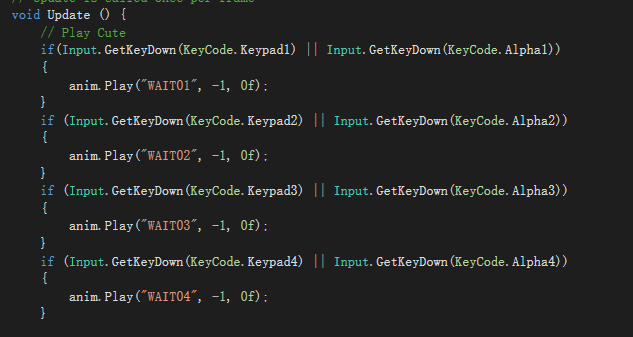
\includegraphics[width=13cm]{code1.png}\\
  \caption{Code1}\label{2-2}
\end{figure}
到这里,基础的动作导入和控制就完成了!
\subsection{混合动画制作}
\paragraph{}
许多模型时自带向前、向后、向左、向右行走的动作,但是对于一个任意的方向,用这些动作来行走将比较奇怪。
Unity中使用\textbf{Blend Tree}的混合动作来实现这一类功能。
\paragraph{}
在\textbf{Animator}面板中创建一个新的\textbf{Blend Tree},命名为\textbf{Walk},将它的\textbf{Blend Type}设置为\textbf{2D Simple Directional}。这样混合的动作将会在一个二维坐标系里根据参数的比例来混合。
\paragraph{}
然后将四个方向的行走动作设置好,并新建两个参数作为混合比例的输入。接着添加两个从\textbf{WAIT00}到\textbf{Walk}的\textbf{Transistion},一个从\textbf{Walk}到\textbf{WAIT00}的\textbf{Transistion}
\begin{figure}[H]
\begin{minipage}{0.5\linewidth}
  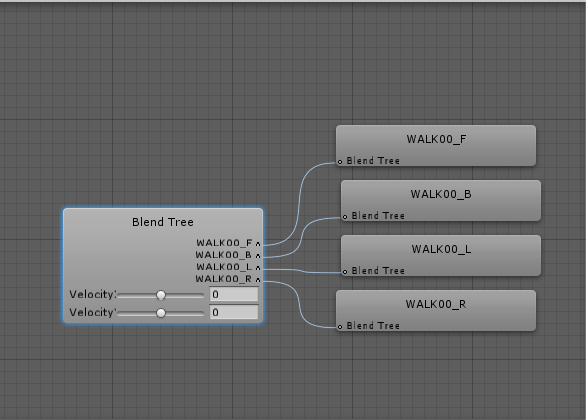
\includegraphics[width=15em]{blend_tree1.png}\\
  \caption{}\label{2-3}
\end{minipage}
\begin{minipage}{0.5\linewidth}
  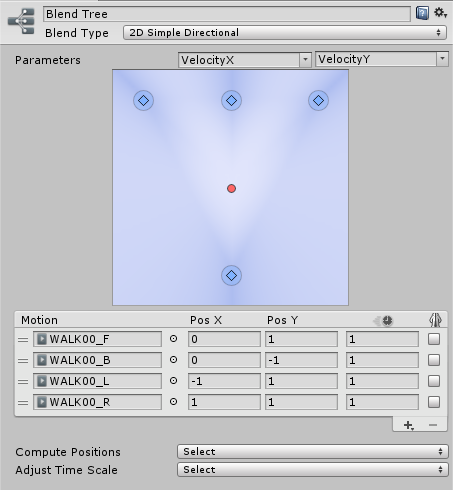
\includegraphics[width=15em]{blend_tree2.png}\\
  \caption{}\label{2-4}
\end{minipage}
\end{figure}
\paragraph{}
我们希望用按键输入来控制行走动画的播放,这需要为\textbf{Walk}状态的转换设置条件。将Y轴的输入大小作为约束条件:如果它是一个大于0.1或者小于-0.1,进入\textbf{Walk}状态,否则回到\textbf{WAIT00}状态。
\paragraph{}
最后在代码中写好输入的接受,并用\textbf{Animator}的\textbf{SetFloat}函数设置状态机中的参数
\begin{figure}[H]
  \centering
  % Requires \usepackage{graphicx}
  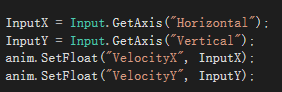
\includegraphics[width=24em]{code2.png}\\
  \caption{}\label{2-5}
\end{figure}
\paragraph{}
然后如法炮制制作了一个\textbf{Run}的动画,使用Left-Shift来控制
\subsection{分层动画}
\paragraph{}
要实现两个不同位置动画同时播放而又不互相干扰,用\textbf{Blend Tree}就不太合适。这种情况需要给状态机设置多层状态,并使用\textbf{Mask}来标记动画改变模型的范围
\begin{figure}[H]
  \centering
  % Requires \usepackage{graphicx}
  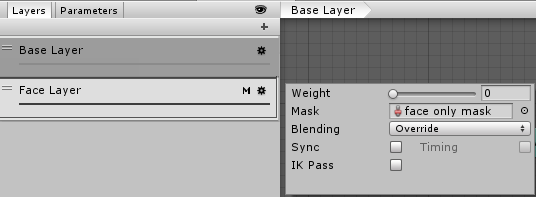
\includegraphics[width=24em]{mask.png}\\
  \caption{}\label{2-6}
\end{figure}
\paragraph{}
使用\textbf{Unity-Chan}中制作好的脸部动作和脸部标记,并且使用\textbf{FaceController}脚本来控制面部表情动画
\begin{figure}[H]
  \centering
  % Requires \usepackage{graphicx}
  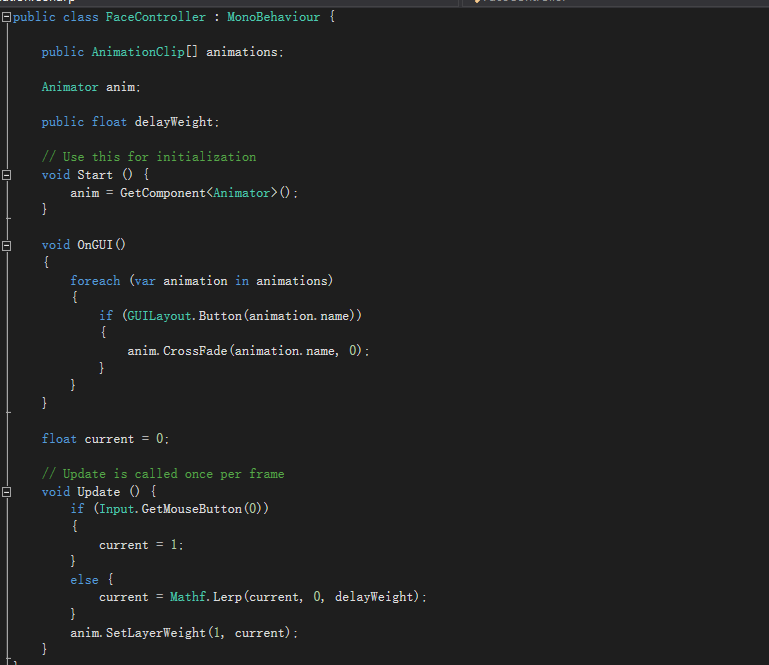
\includegraphics[width=30em]{code3.png}\\
  \caption{}\label{2-7}
\end{figure}
\paragraph{}
这样即可实现脸部动作和身体动作同时播放而又不互相影响的效果。
\begin{figure}[H]
\begin{minipage}{0.5\linewidth}
  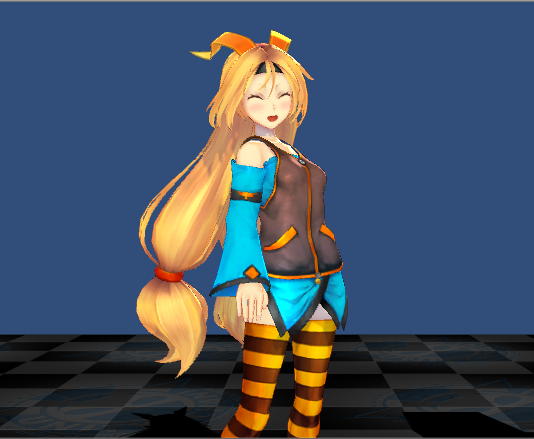
\includegraphics[width=15em]{face.png}\\
  \caption{}\label{2-8}
\end{minipage}
\begin{minipage}{0.5\linewidth}
  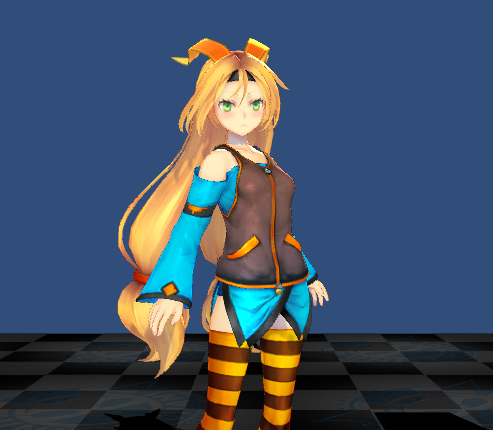
\includegraphics[width=15em]{face1.png}\\
  \caption{}\label{2-9}
\end{minipage}
\end{figure}
\section{物品动画}
\subsection{制作}
使用Blender的动画功能制作简单的物体动画\textbf{MagicCube}。动画的主题是一个2X2X2的魔方,首先创建8个Cube排列成魔方。然后在时间轴上选中帧数,移动、旋转或者改变Cube的大小,然后插入关键帧。制作完成后导出.FBX文件拖入Unity里即可使用。
\subsection{控制}
由于导出时设定了将动画合并成一个Action,所以模型虽然有8个方块,但是控制起来十分方便。
\begin{figure}[H]
  \centering
  % Requires \usepackage{graphicx}
  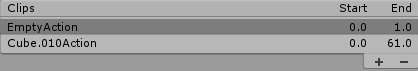
\includegraphics[width=18em]{clips.png}\\
  \caption{}\label{3-1}
\end{figure}
在Unity的assets中可以看到导入的动画带有两个\textbf{Clips},即两个动画切片,可以分开使用。\textbf{EmptyAction}是一个空的动作,什么也没做,而\textbf{Cube.010Action}就是刚刚制作好的动画。
\paragraph{}
制作一个简单的状态机\textbf{Animator}控制这个模型即可。
\begin{figure}[H]
  \centering
  % Requires \usepackage{graphicx}
  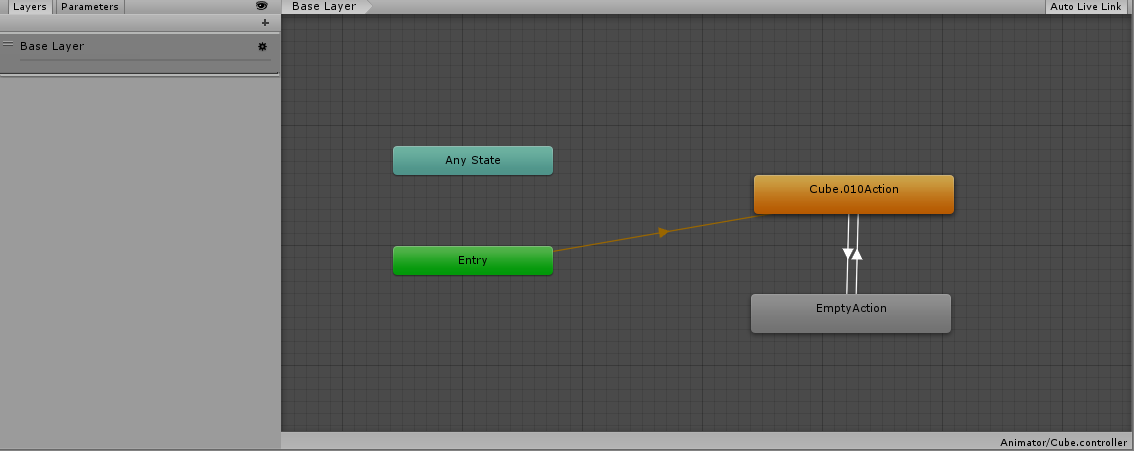
\includegraphics[width=24em]{cubeController.png}\\
  \caption{}\label{3-2}
  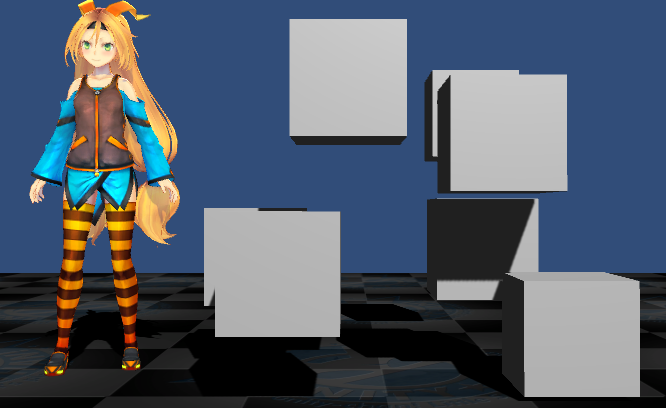
\includegraphics[width=24em]{result.png}\\
  \caption{}\label{3-3}
\end{figure}
\newpage
\section{总结}
\paragraph{}
这次作业让我学到了建模软件动画的制作和Unity对导入动画的控制,熟悉了动画控制的整个流程,并对\textbf{Blend Tree}、\textbf{Mask}等机制有所了解,也稍微熟悉了Blender的操作。
\paragraph{}
实际上最开始我准备自己做一个人物(双足)模型来完成这次作业的,结果建模就用了我3天时间,结果做好了骨架没时间做动画,果然建模是个功夫活。希望我的模型能出现在后面的游戏大作业中。
\begin{figure}[H]
  \centering
  % Requires \usepackage{graphicx}
  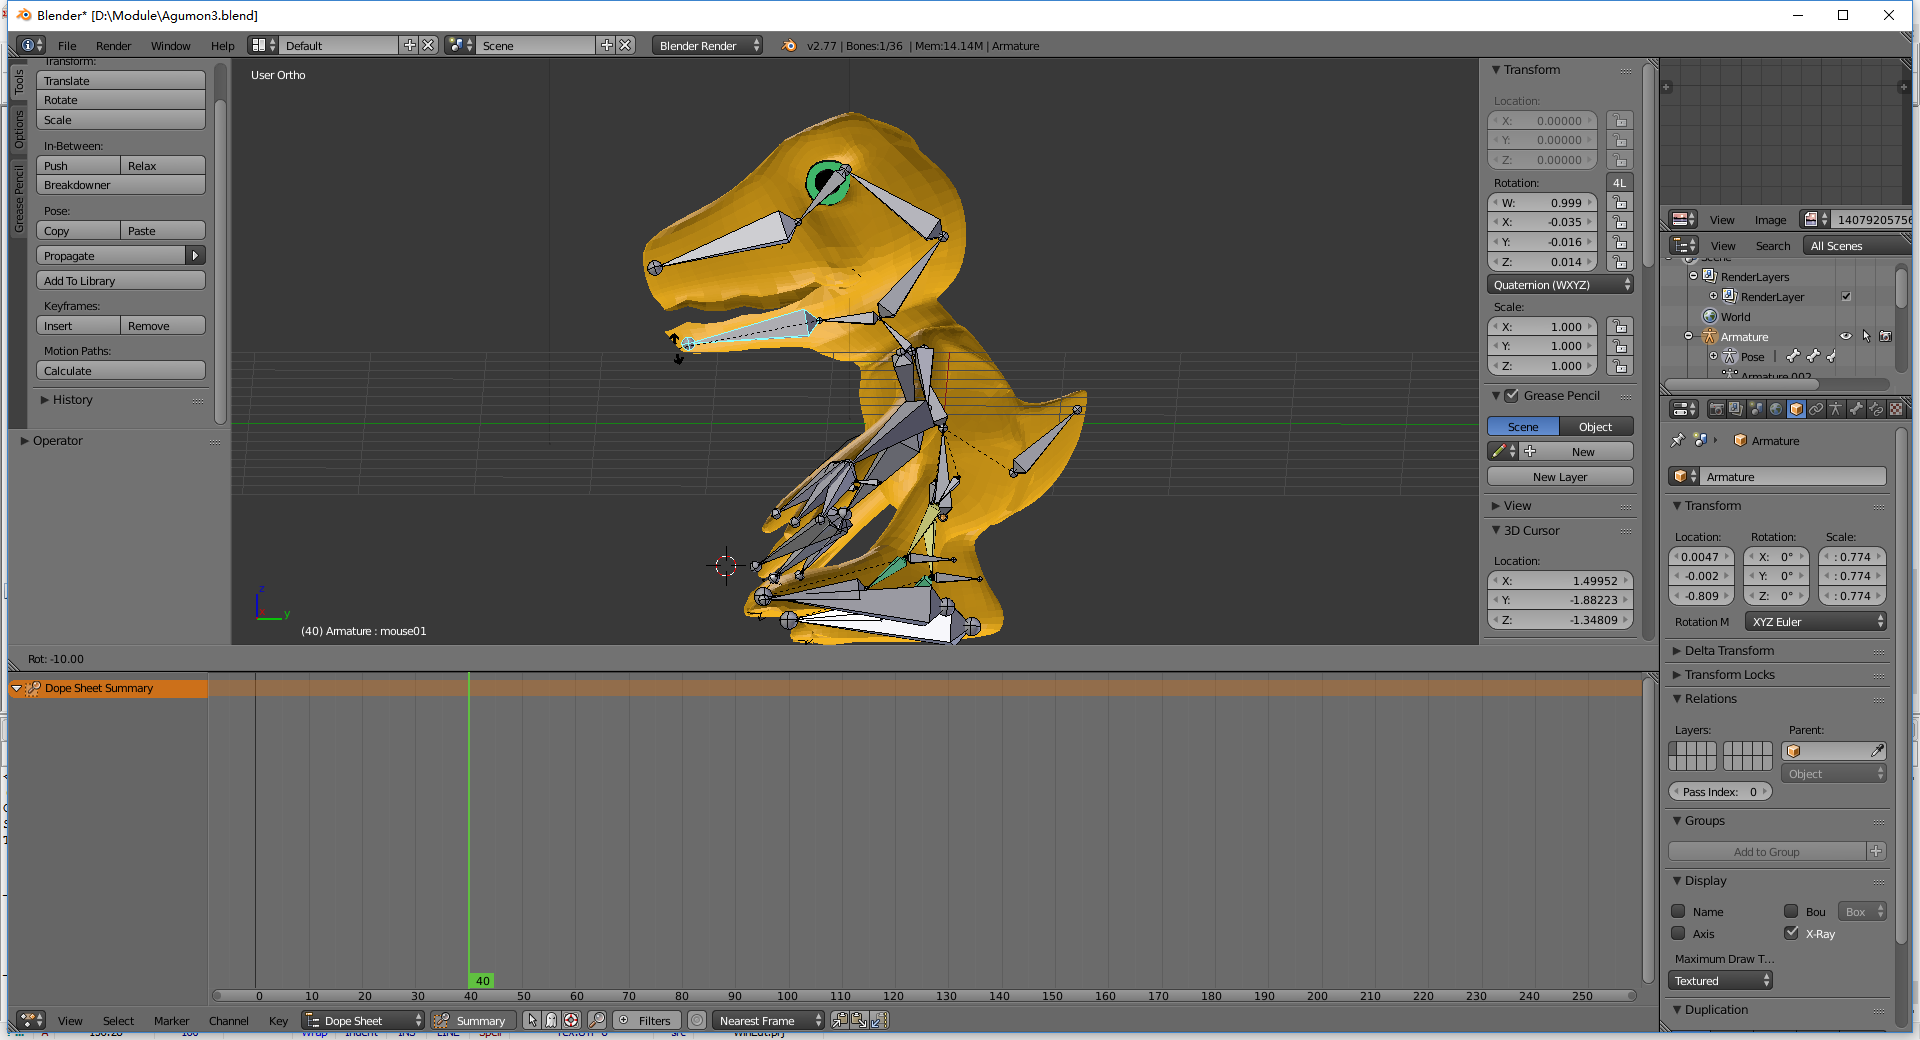
\includegraphics[width=30em]{Agumon.png}\\
  \caption{未完成的亚古兽}\label{4-1}
\end{figure}

\end{document}
